\documentclass[tikz,border=0pt]{standalone}
\usepackage[T1]{fontenc}
\usepackage{tgheros}
\usepackage{graphicx}
\usepackage{newtxmath}
\usepackage{amsmath}
\usetikzlibrary{arrows.meta}
\renewcommand{\familydefault}{\sfdefault}

\definecolor{ink}{HTML}{172C3D}
\definecolor{muted}{HTML}{526674}
\definecolor{edge}{HTML}{B9C9D4}
\definecolor{teal}{HTML}{147D75}
\definecolor{tea}{HTML}{EAF6F3}
\definecolor{amber}{HTML}{9B5C21}
\definecolor{cream}{HTML}{FFF4E7}
\definecolor{bluegray}{HTML}{EDF3F8}
\definecolor{soft}{HTML}{F7F9FB}

\begin{document}
\begin{tikzpicture}[
  x=1mm,y=1mm,text=ink,font=\sffamily\fontsize{8.2}{10}\selectfont,
  heading/.style={anchor=west,inner sep=0pt,font=\sffamily\bfseries\fontsize{9.5}{11}\selectfont},
  left/.style={anchor=west,inner sep=0pt},
  right/.style={anchor=east,inner sep=0pt},
  detail/.style={font=\sffamily\fontsize{7.7}{9.2}\selectfont,text=muted,inner sep=0pt},
  flow/.style={-{Stealth[length=1.35mm,width=1.15mm]},draw=muted,line width=.65pt},
  marker/.style={circle,draw=ink,fill=white,inner sep=0pt,minimum size=1.65mm,line width=.60pt},
  chip/.style={rounded corners=1pt,inner xsep=2.8pt,inner ysep=2pt},
  card/.style={draw=edge,line width=.48pt,rounded corners=1.7pt,fill=soft}
]
\path[use as bounding box] (0,0) rectangle (122,-91);
\node[heading] at (1,-3) {(a)\enspace Reconstruct the budget at close $t$};
\node[detail,right] at (121,-3) {Illustrative stock example};

% Time axis contrasts the observed interval at s with the decision at t.
\draw[flow] (2,-13.2) -- (120.5,-13.2);
\draw[amber,line width=1.25pt] (12,-13.2) -- (43,-13.2);
\node[marker] at (12,-13.2) {};
\node[marker] at (43,-13.2) {};
\node[marker,fill=ink] at (113,-13.2) {};
\node at (12,-9.3) {Close $s-1$};
\node at (43,-9.3) {Close $s$};
\node at (113,-9.3) {Close $t$};
\fill[white] (70,-14.35) rectangle (74,-12);
\draw[muted,line width=.55pt] (70.9,-14.25) -- (72.4,-12.05)
  (72.05,-14.25) -- (73.55,-12.05);

\node[chip,fill=tea] (past) at (11.7,-21.5) {Prior tilt $\tau_{i,s-1}$};
\node[chip,fill=cream] (price) at (42.7,-21.5) {Observed return $r^{\mathrm{obs}}_{i,s}$};
\draw[teal,line width=.55pt] (12,-14.2) -- (12,-18.8);
\draw[amber,line width=.55pt] (43,-14.2) -- (43,-18.8);
\node[chip,fill=bluegray,left] (pair) at (61,-21.5)
  {Unscaled return $\displaystyle\tilde r_s=\tfrac{1}{|\mathcal B_s|}\sum_{i\in\mathcal B_s}\tau_{i,s-1}r^{\mathrm{obs}}_{i,s}$};

% The two measured inputs join in a shared connector below the row.
\draw[muted,line width=.55pt] (past.south) |- (42.7,-26.8) -- (price.south);
\draw[flow] (42.7,-26.8) -- (58.1,-26.8) |- (pair.west);

% These illustrative daily returns in percent yield about 25% annualised
% population volatility at 252 trading days, as in the overview figure.
\draw[card,fill=cream!48] (1,-30.5) rectangle (83,-59.4);
\node[left,font=\bfseries] at (4,-34.8) {Trailing 20 unscaled returns};
\node[anchor=south west,inner sep=0pt] at (3.55,-58.65)
  {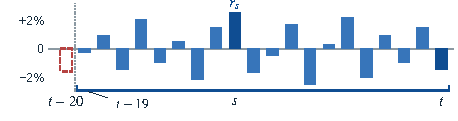
\includegraphics{voltilt_figure_panels/returns_window.pdf}};

\draw[card,fill=bluegray] (88,-30.5) rectangle (121,-59.4);
\draw[flow,draw=amber] (83,-45.2) -- (88,-45.2);
\node[font=\sffamily\bfseries\fontsize{7.6}{9}\selectfont] at (104.5,-34.8) {Annualised volatility};
\node at (104.5,-39.6) {$\hat\sigma_t=25\%$};
\draw[edge,line width=.45pt] (91,-43.3) -- (118,-43.3);
\node[font=\bfseries] at (104.5,-47.5) {Invested fraction};
\node[font=\fontsize{9}{10}\selectfont] at (104.5,-53.35)
  {$\lambda_t=20\%/25\%=0.80$};

\node[detail,left] at (1,-63.1)
  {The tilt chosen at close $t$ can enter the volatility estimate only after a later return is observed.};

% Fix the same budget for both compositions. Values are percentages of capital.
\node[heading] at (1,-69.3) {(b)\enspace Match the daily budget};
\node[detail,right] at (121,-69.3) {Same $\lambda_t^{\mathrm{ref}}=0.80$ in both portfolios};
\draw[card] (1,-73) rectangle (59.9,-90.7);
\draw[card] (62.1,-73) rectangle (121,-90.7);
\node[left,font=\bfseries] at (4,-76.6) {Equal weights};
\node[left,font=\bfseries] at (65.1,-76.6) {News ranks};
\node[detail,right] at (56.9,-76.6) {$\boldsymbol q_t=(1,1,1)/3$};
\node[detail,right] at (118,-76.6) {$\boldsymbol q_t=(1.5,1,0.5)/3$};

\node[anchor=south west,inner sep=0pt] at (4,-87.3)
  {
\includegraphics{voltilt_figure_panels/capital_equal.pdf}};
\node[anchor=south west,inner sep=0pt] at (65.1,-87.3)
  {
\includegraphics{voltilt_figure_panels/capital_tilted.pdf}};
\end{tikzpicture}
\end{document}
